\documentclass[a4paper]{article}
\usepackage{times}
\usepackage[utf8]{inputenc}
\usepackage[T1]{fontenc}
\usepackage{selinput}
\usepackage{upquote}
\usepackage[margin=2cm, rmargin=4cm, tmargin=3cm]{geometry}
\usepackage{tcolorbox}
\usepackage{xspace}
\usepackage{amsmath}
\usepackage{float}
\usepackage[french]{babel}
\usepackage{hyperref}
\usepackage{xurl}
\usepackage{fontawesome6}
\usepackage{enumitem}
\usepackage{marginnote}
\usepackage{ulem}
\usepackage[yyyymmdd,hhmmss]{datetime}
\usepackage{ulem}
\usepackage{environ}
\usepackage{graphicx}
%\usepackage[top=Bcm, bottom=Hcm, outer=Ccm, inner=Acm, heightrounded, marginparwidth=Ecm, marginparsep=Dcm]{geometry}
\usepackage{courier}



\newtcolorbox{Example}[1]{colback=white,left=20pt,colframe=slideblue,fonttitle=\bfseries,title=#1}
\newtcolorbox{Solutions}[1]{colback=white,left=20pt,colframe=green,fonttitle=\bfseries,title=#1}
\newtcolorbox{Conseils}[1]{colback=white,left=20pt,colframe=slideblue,fonttitle=\bfseries,title=#1}
\newtcolorbox{Warning}[1]{colback=white,left=20pt,colframe=warning,fonttitle=\bfseries,title=#1}
\newtcolorbox{Note}[1]{colback=white,left=20pt,colframe=grey,fonttitle=\bfseries,title=#1}
\newtcolorbox{Dessin}[1]{colback=white,left=20pt,colframe=grey,fonttitle=\bfseries,title=#1}

\setlength\parindent{0pt}

  %Exercice environment
  \newcounter{exercice}
  \newenvironment{Exercice}[1][]
  {
  \par
  \stepcounter{exercice}\textbf{Question \arabic{exercice}:} (\faClock \enskip \textit{#1})
  }
  {\bigskip}
  

% Title
\newcommand{\titre}{\begin{center}
  \section*{Algorithmes et Pensée Computationnelle}
\end{center}}
\newcommand{\cours}[1]
{\begin{center} 
  \textit{#1}\\
\end{center}
  }



% \newcommand{\exemple}[1]{\newline~\textbf{Exemple :} #1}
\newcommand{\todo}[1]{\textcolor{red}{#1}}
%\newcommand{\attention}[1]{\newline\faExclamationTriangle~\textbf{Attention :} #1}

% Documentation url (escape \# in the TP document)
\newcommand{\documentation}[1]{\faBookOpen~Documentation : \href{#1}{#1}}

% Clef API
\newcommand{\apikey}[1]{\faKey~Clé API : \lstinline{#1}}
\newcommand{\apiendpoint}[1]{\faGlobe~Url de base de l'API \href{#1}{#1}}

%Listing Python style
\usepackage{color}
\definecolor{slideblue}{RGB}{33,131,189}
\definecolor{green}{RGB}{0,190,100}
\definecolor{blue}{RGB}{121,142,213}
\definecolor{grey}{RGB}{120,120,120}
\definecolor{warning}{RGB}{235,186,1}

\usepackage{listings}
\lstdefinelanguage{texte}{
    keywordstyle=\color{black},
    numbers=none,
    frame=none,
    literate=
           {é}{{\'e}}1
           {è}{{\`e}}1
           {ê}{{\^e}}1
           {à}{{\`a}}1
           {â}{{\^a}}1
           {ù}{{\`u}}1
           {ü}{{\"u}}1
           {î}{{\^i}}1
           {ï}{{\"i}}1
           {ë}{{\"e}}1
           {Ç}{{\,C}}1
           {ç}{{\,c}}1
           {ô}{{\^o}}1,
    columns=fullflexible,keepspaces,
	breaklines=true,
	breakatwhitespace=true,
}
\lstset{
  language=Python,
	%basicstyle=\bfseries\footnotesize,
  basicstyle=\footnotesize\ttfamily\small,
	breaklines=true,
	breakatwhitespace=true,
	commentstyle=\color{grey},
	stringstyle=\color{slideblue},
  keywordstyle=\color{slideblue},
	morekeywords={with, as, True, False, Fraction, Float, join, index, None, main, argparse, self, sort, __eq__, __add__, __mul__ ,__ne__, __radd__, __del__, __ge__, __gt__, split, os, endswith, is_file, scandir, @classmethod, this},
	deletekeywords={id},
	showspaces=false,
	showstringspaces=false,
	columns=fullflexible,keepspaces,
	literate=
           {é}{{\'e}}1
           {è}{{\`e}}1
           {ê}{{\^e}}1
           {à}{{\`a}}1
           {â}{{\^a}}1
           {ù}{{\`u}}1
           {ü}{{\"u}}1
           {î}{{\^i}}1
           {ï}{{\"i}}1
           {ë}{{\"e}}1
           {Ç}{{\,C}}1
           {ç}{{\,c}}1
           {ô}{{\^o}}1,
    numbers=left,
}

\newtcbox{\mybox}{nobeforeafter,colframe=white,colback=slideblue,boxrule=0.5pt,arc=1.5pt, boxsep=0pt,left=2pt,right=2pt,top=2pt,bottom=2pt,tcbox raise base}
\newcommand{\projet}{\mybox{\textcolor{white}{\small projet}}\xspace}
\newcommand{\optionnel}{\mybox{\textcolor{white}{\small Optionnel}}\xspace}
\newcommand{\advanced}{\mybox{\textcolor{white}{\small Pour aller plus loin}}\xspace}
\newcommand{\auto}{\mybox{\textcolor{white}{\small Auto-évaluation}}\xspace}


\usepackage{environ}
\newif\ifShowSolution
\NewEnviron{solution}{
  \ifShowSolution
	\begin{Solutions}{\faTerminal \enskip Solution}
		\BODY
	\end{Solutions}
  \fi}

\usepackage{environ}
\newif\ifShowExample
\NewEnviron{exemple}{
  \ifShowExample
	\begin{Example}{\faTerminal \enskip Exemple}
		\BODY
	\end{Example}
  \fi}

\usepackage{environ}
 \newif\ifShowConseil
  \NewEnviron{conseil}{
    \ifShowConseil
    \begin{Conseils}{\faLightbulb \quad Conseil}
      \BODY
    \end{Conseils}

    \fi}

    \usepackage{environ}
  \newif\ifShowWarning
  \NewEnviron{attention}{
    \ifShowWarning
    \begin{Warning}{\faTriangleExclamation \quad Attention}
      \BODY
    \end{Warning}

    \fi}

  \newif\ifShowNote
  \NewEnviron{note}[1]{
    \ifShowNote
    \begin{Note}{\faEye \quad Comment added by #1 at \date - \currenttime}
      \BODY
    \end{Note}

    \fi}  

    \newif\ifShowDessin
    \NewEnviron{dessin}[1]{
      \ifShowDessin
      \begin{Dessin}{\faPen \quad Figure}
        \BODY
      \end{Dessin}
  
      \fi}  

%\newcommand{\Conseil}[1]{\ifShowIndice\ \newline\faLightbulb[regular]~#1\fi}

\usepackage{tikz}
\usetikzlibrary{arrows.meta}
\graphicspath{{img/}}

% Les coordonnées des flèches sont relatives à chaque capture d'écran.
\definecolor{noticearrow}{RGB}{204,72,32}
\tikzset{
  notice arrow/.style={draw=noticearrow, line width=2.2pt,
    -{Stealth[length=4mm]}},
  notice badge/.style={circle, draw=noticearrow, line width=1pt,
    fill=white, text=noticearrow, font=\bfseries\small,
    inner sep=1pt, minimum size=5.5mm}
}
\newcommand{\stepmark}[5]{%
  \node[notice badge] (step#1) at (#2,#3) {#1};
  \draw[notice arrow] (step#1) -- (#4,#5);
}
\newcommand{\shotcaption}[1]{\par\smallskip{\small\itshape #1}\par\medskip}

\begin{document}
\titre
\cours{Premiers pas avec Java dans IntelliJ IDEA}

\textit{NB: Il est recommandé de commencer avec le tutoriel sur Python avant ce tutoriel}. La semaine dernière, vous avez appris à créer et à exécuter des programmes depuis la ligne de commande, notamment en leur passant des arguments. Cette semaine, vous allez voir comment réaliser ces mêmes tâches directement dans IntelliJ IDEA.

\section{Créer un projet Java dans IntelliJ IDEA}

Sur l'écran d'accueil, sélectionnez \textbf{New Project}. Si un projet est déjà
ouvert, utilisez \textbf{File $>$ New $>$ Project}. Dans la fenêtre de création,
choisissez \textbf{Java} (1), donnez un nom et un emplacement au projet (2),
laissez \textbf{IntelliJ} comme système de construction, puis sélectionnez un
\textbf{JDK} installé (3). Le numéro de version et les chemins affichés peuvent
être différents sur votre machine. Laissez \textbf{Add sample code} décoché,
comme sur la capture, et cliquez sur \textbf{Create} (4).

\begin{center}
\begin{tikzpicture}
  \node[anchor=south west,inner sep=0] (screen) at (0,0)
    {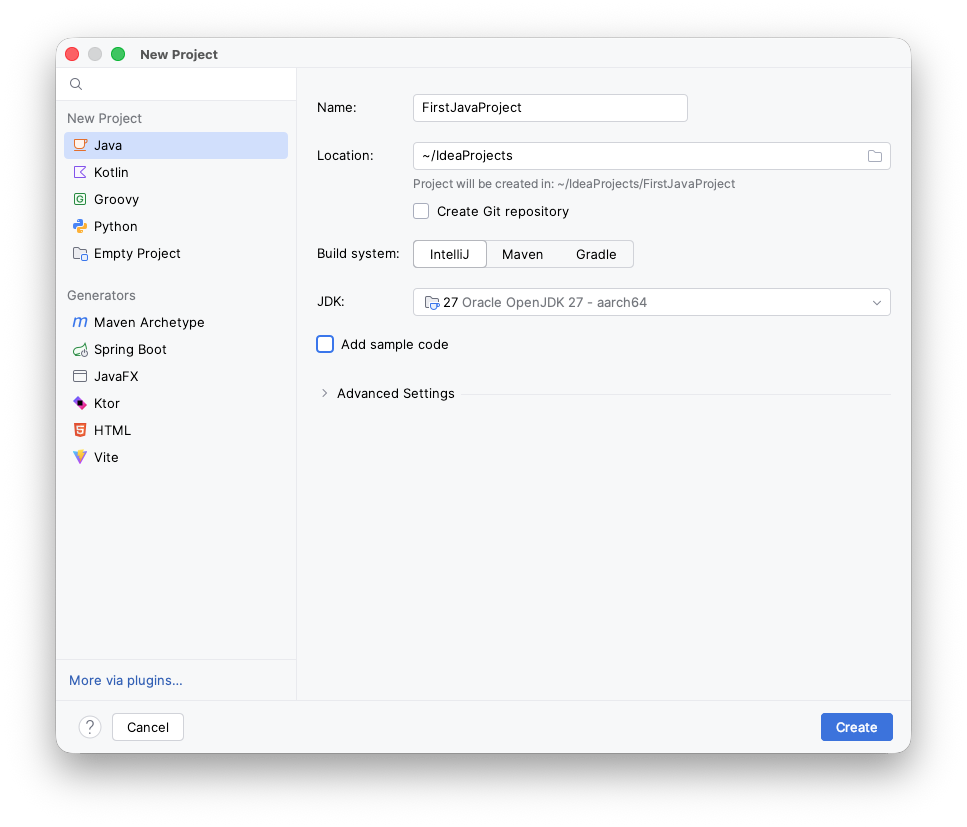
\includegraphics[width=.80\linewidth]{creatingProject.png}};
  \begin{scope}[x={(screen.south east)},y={(screen.north west)}]
    \stepmark{1}{.34}{.78}{.15}{.825}
    \stepmark{2}{.78}{.88}{.57}{.87}
    \stepmark{3}{.79}{.57}{.57}{.635}
    \stepmark{4}{.69}{.15}{.89}{.12}
  \end{scope}
\end{tikzpicture}
\shotcaption{Choisissez Java, nommez le projet, vérifiez le JDK et créez le projet.}
\end{center}

\clearpage
\subsection*{Créer la classe Main}

Dans le panneau \textbf{Project}, faites un clic droit sur le dossier
\lstinline{src} (1). Dans le menu contextuel, choisissez \textbf{New} (2),
puis \textbf{Java Class} (3). Les deux menus ci-dessous sont replacés sur la
fenêtre du projet dans leur ordre de superposition.

\begin{center}
\begin{tikzpicture}
  \node[anchor=south west,inner sep=0] (screen) at (0,0)
    {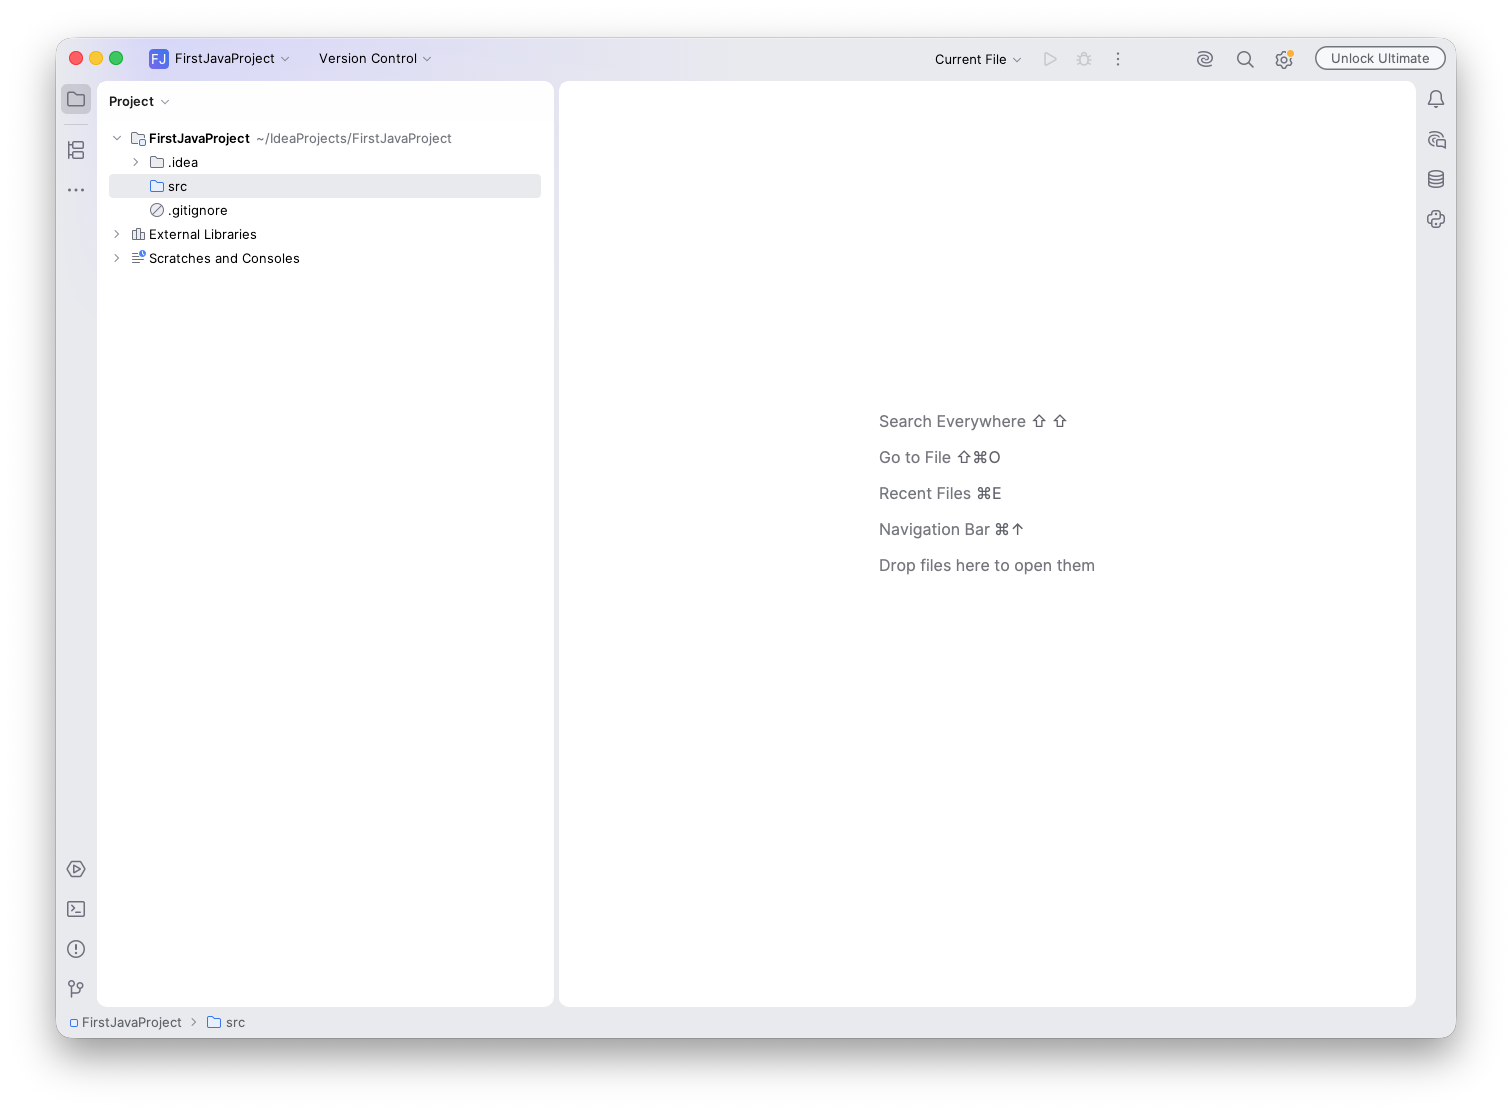
\includegraphics[width=\linewidth]{leftmostSubwindow.png}};
  \begin{scope}[x={(screen.south east)},y={(screen.north west)}]
    % Même échelle que la capture 1512 x 1112 : les bordures noires des
    % captures de menus sont rognées avant de les superposer.
    \node[anchor=north west,inner sep=0] at (.130,.84)
      {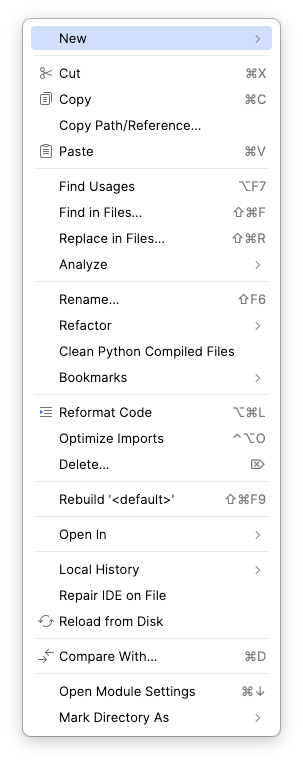
\includegraphics[trim=23 19 23 20,clip,width=.170\linewidth]
        {middleSubwindow.png}};
    \node[anchor=north west,inner sep=0] at (.298,.84)
      {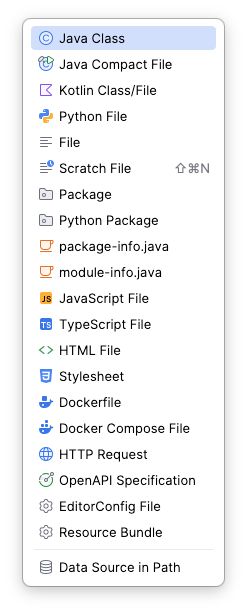
\includegraphics[trim=23 19 23 19,clip,width=.133\linewidth]
        {rightmostSubwindow.png}};
    \stepmark{1}{.085}{.92}{.115}{.833}
    \stepmark{2}{.27}{.94}{.175}{.815}
    \stepmark{3}{.49}{.94}{.35}{.815}
  \end{scope}
\end{tikzpicture}
\shotcaption{Clic droit sur src, puis New et Java Class.}
\end{center}

Saisissez \lstinline{Main} comme nom (1), conservez le type \textbf{Class}
(2), puis appuyez sur Entrée. IntelliJ crée le fichier \lstinline{Main.java}
dans le dossier \lstinline{src}.

\begin{center}
\begin{tikzpicture}
  \node[anchor=south west,inner sep=0] (screen) at (0,0)
    {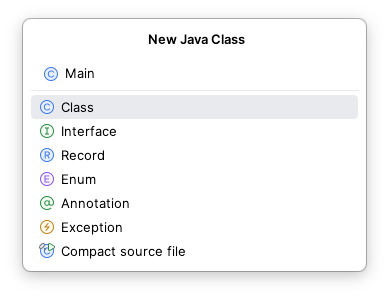
\includegraphics[width=.49\linewidth]{specifyClassName.png}};
  \begin{scope}[x={(screen.south east)},y={(screen.north west)}]
    \stepmark{1}{.78}{.80}{.22}{.75}
    \stepmark{2}{.77}{.38}{.22}{.64}
  \end{scope}
\end{tikzpicture}
\shotcaption{Nommez la classe Main et laissez Class sélectionné.}
\end{center}

\clearpage
Le nouveau fichier apparaît dans le panneau \textbf{Project} (1) et s'ouvre
dans l'éditeur (2). IntelliJ a déjà écrit la déclaration de la classe et ses
accolades. Le code que vous ajouterez doit être placé \emph{entre} ces deux
accolades.

\begin{center}
\begin{tikzpicture}
  \node[anchor=south west,inner sep=0] (screen) at (0,0)
    {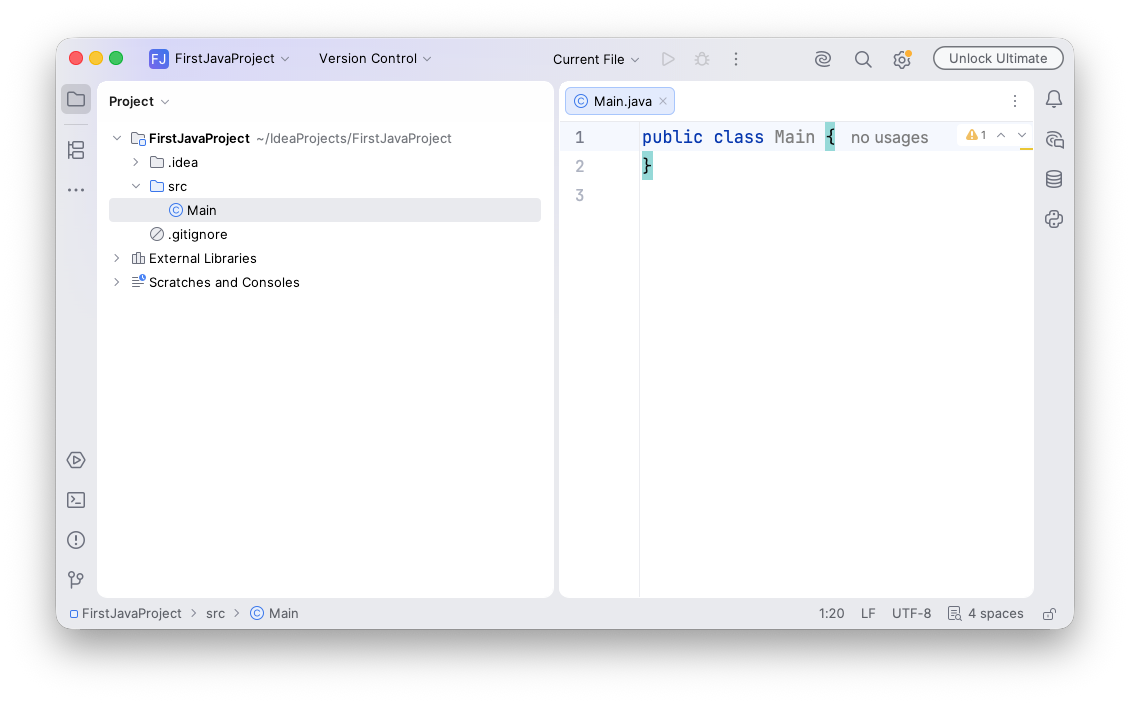
\includegraphics[width=.79\linewidth]{classCreated.png}};
  \begin{scope}[x={(screen.south east)},y={(screen.north west)}]
    \stepmark{1}{.35}{.75}{.18}{.70}
    \stepmark{2}{.83}{.69}{.62}{.80}
  \end{scope}
\end{tikzpicture}
\shotcaption{Le fichier Main.java et le corps encore vide de sa classe.}
\end{center}

\section{Créer des variables}

Pour lancer une application Java, ajoutez dans la classe la méthode
ci-dessous (1). Elle constitue le point d'entrée du programme.
\begin{center}
\lstinline{public static void main(String[] args)}
\end{center}
Dans ses accolades, écrivez \lstinline{int a = 1;}
(2). Le mot \lstinline{int} indique que \lstinline{a} contient un nombre
entier ; le signe \lstinline{=} lui attribue la valeur \lstinline{1}.
Terminez chaque instruction par un point-virgule. La ligne suivante (3)
affiche la valeur de \lstinline{a} :
\begin{center}
\lstinline{System.out.print(a);}
\end{center}

\begin{center}
\begin{tikzpicture}
  \node[anchor=south west,inner sep=0] (screen) at (0,0)
    {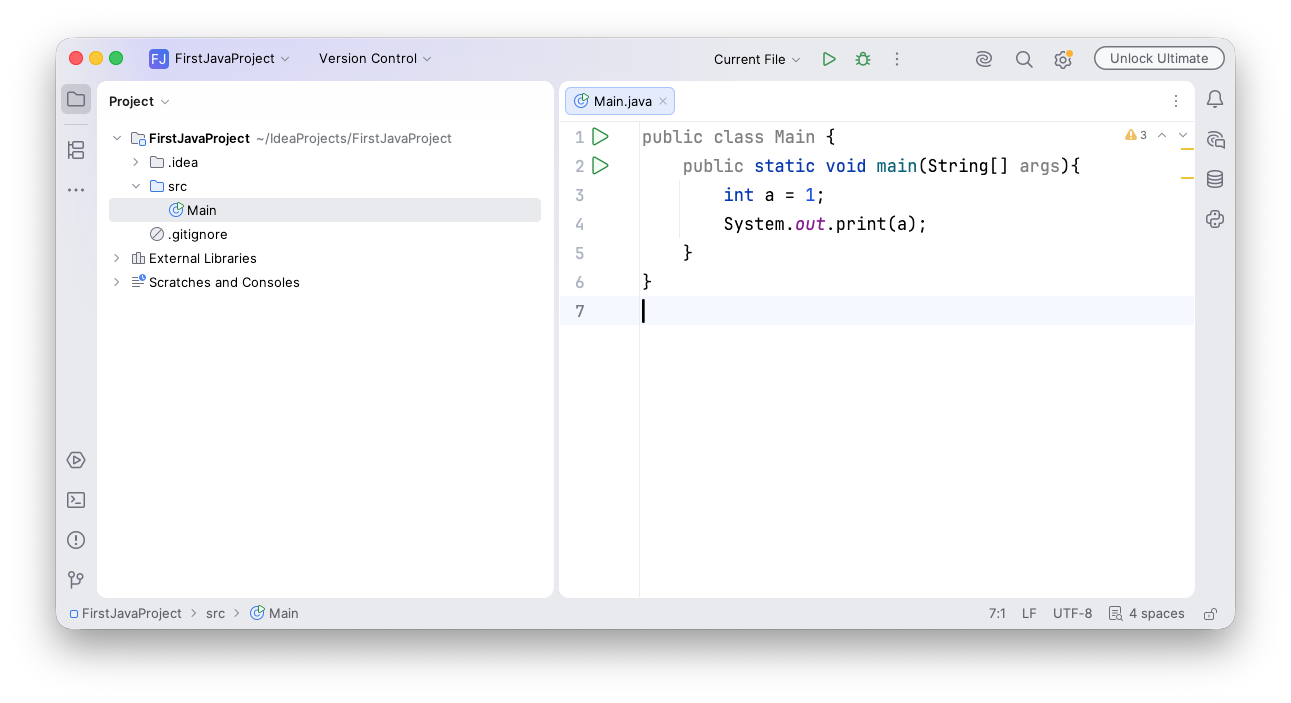
\includegraphics[width=.93\linewidth]{creatingVariables.png}};
  \begin{scope}[x={(screen.south east)},y={(screen.north west)}]
    \stepmark{1}{.83}{.79}{.70}{.766}
    \stepmark{2}{.84}{.68}{.62}{.723}
    \stepmark{3}{.83}{.55}{.64}{.680}
  \end{scope}
\end{tikzpicture}
\shotcaption{La méthode main, la déclaration d'une variable entière et son affichage.}
\end{center}

Pour essayer d'autres types, écrivez
\lstinline{String message = "Bonjour";} pour du texte.
La déclaration \lstinline{boolean actif = true;} représente une valeur vraie
ou fausse. Placez ces lignes à l'intérieur de \lstinline{main}.
Cliquez sur le triangle vert à côté de
\lstinline{main}, puis choisissez \textbf{Run 'Main.main()'}. Le panneau
\textbf{Run} affiche \lstinline{1} pour le programme de la capture.

\clearpage
\section{Les arguments de la ligne de commande}

Les arguments permettent de transmettre des valeurs au programme lors de son
lancement. La méthode \lstinline{main} les reçoit dans le tableau
\lstinline{String[] args} (1). Remplacez les deux instructions de l'exemple
précédent par la ligne suivante (2) :
\begin{center}
\lstinline{System.out.print(args[0]);}
\end{center}
En Java,
\lstinline{args[0]} est le \emph{premier} argument fourni ;
\lstinline{args[1]} serait le deuxième.

\begin{center}
\begin{tikzpicture}
  \node[anchor=south west,inner sep=0] (screen) at (0,0)
    {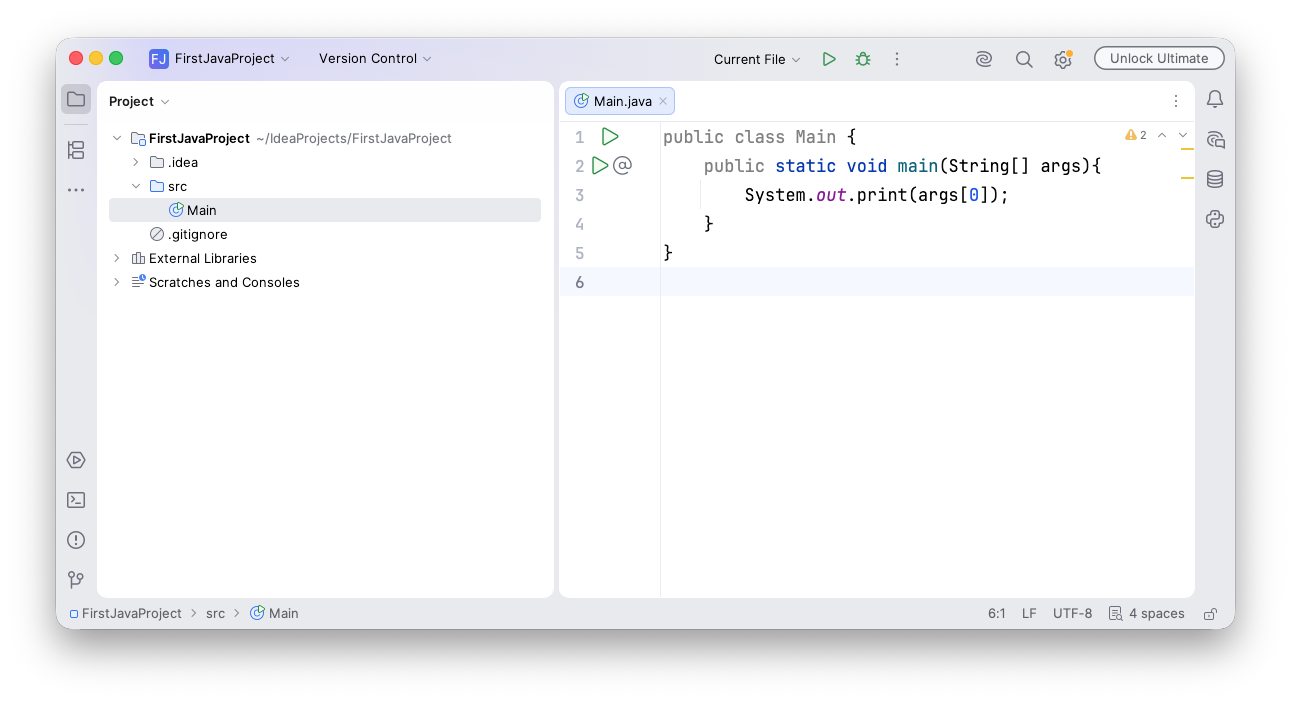
\includegraphics[width=.93\linewidth]{programWithParameters.png}};
  \begin{scope}[x={(screen.south east)},y={(screen.north west)}]
    \stepmark{1}{.87}{.79}{.81}{.765}
    \stepmark{2}{.84}{.55}{.75}{.722}
  \end{scope}
\end{tikzpicture}
\shotcaption{Le tableau args reçoit les arguments et args[0] désigne le premier.}
\end{center}

Après un premier lancement avec le triangle vert à côté de \lstinline{main},
ouvrez \textbf{Run $>$ Edit Configurations...} et sélectionnez la configuration
\textbf{Main}. Dans le champ des arguments de l'application, saisissez
\lstinline{FirstParam} (1), puis cliquez sur \textbf{Run} (2). IntelliJ
transmet ce mot à \lstinline{args[0]} et le programme l'affiche dans le panneau
\textbf{Run}. Si vous fournissez plusieurs mots séparés par des espaces, ils
occupent les positions \lstinline{args[0]}, \lstinline{args[1]}, etc. Il faut
fournir au moins un argument avant de lancer le code de la capture.

\begin{center}
\begin{tikzpicture}
  \node[anchor=south west,inner sep=0] (screen) at (0,0)
    {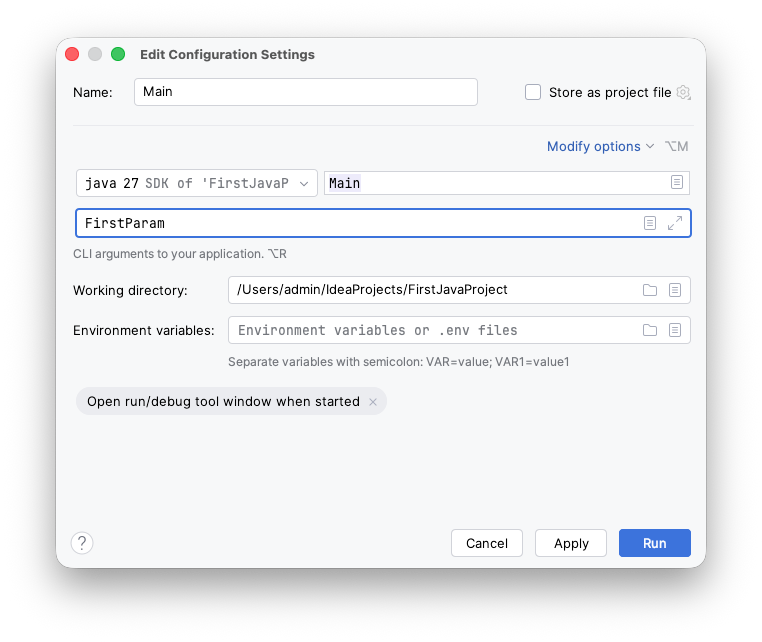
\includegraphics[width=.69\linewidth]{specifyParams.png}};
  \begin{scope}[x={(screen.south east)},y={(screen.north west)}]
    \stepmark{1}{.71}{.75}{.26}{.652}
    \stepmark{2}{.69}{.28}{.86}{.154}
  \end{scope}
\end{tikzpicture}
\shotcaption{Entrez FirstParam dans les arguments de l'application, puis lancez Main.}
\end{center}

\end{document}
